\documentclass[sigconf]{acmart}
% =============================================================================
% Template setup — participants normally do not edit this file.
% Author content belongs in main.tex; citations belong in main.bib.
% \documentclass lives in main.tex so Overleaf does not treat this file as root.
% =============================================================================

% --- Competition / non-ACM-submission friendly rights metadata ------------
\setcopyright{none}
\settopmatter{printacmref=false}
\acmConference[Kaggle Competition]{Filament Segmentation Challenge}{2026}{\href{https://www.kaggle.com/competitions/filament-segmentation-2026}{kaggle.com/competitions/filament-segmentation-2026}}
\acmBooktitle{Competition Report}
\acmDOI{}
\acmISBN{}

% --- Author guidance text --------------------------------------------------
% \guide{...} is gray italic while \guideStyletrue; omitted from the PDF if false.
% Flip the switch in main.tex after % =============================================================================
% Template setup — participants normally do not edit this file.
% Author content belongs in main.tex; citations belong in main.bib.
% \documentclass lives in main.tex so Overleaf does not treat this file as root.
% =============================================================================

% --- Competition / non-ACM-submission friendly rights metadata ------------
\setcopyright{none}
\settopmatter{printacmref=false}
\acmConference[Kaggle Competition]{Filament Segmentation Challenge}{2026}{\href{https://www.kaggle.com/competitions/filament-segmentation-2026}{kaggle.com/competitions/filament-segmentation-2026}}
\acmBooktitle{Competition Report}
\acmDOI{}
\acmISBN{}

% --- Author guidance text --------------------------------------------------
% \guide{...} is gray italic while \guideStyletrue; omitted from the PDF if false.
% Flip the switch in main.tex after % =============================================================================
% Template setup — participants normally do not edit this file.
% Author content belongs in main.tex; citations belong in main.bib.
% \documentclass lives in main.tex so Overleaf does not treat this file as root.
% =============================================================================

% --- Competition / non-ACM-submission friendly rights metadata ------------
\setcopyright{none}
\settopmatter{printacmref=false}
\acmConference[Kaggle Competition]{Filament Segmentation Challenge}{2026}{\href{https://www.kaggle.com/competitions/filament-segmentation-2026}{kaggle.com/competitions/filament-segmentation-2026}}
\acmBooktitle{Competition Report}
\acmDOI{}
\acmISBN{}

% --- Author guidance text --------------------------------------------------
% \guide{...} is gray italic while \guideStyletrue; omitted from the PDF if false.
% Flip the switch in main.tex after \input{preamble}.
%
% Do not use \guide{...} for \email{...}.
\usepackage{xcolor}
\newif\ifguideStyle
\guideStyletrue
\newcommand{\guide}[1]{%
  \ifguideStyle
    {\color{gray!65}\itshape #1}%
  \fi
}

% --- Math ------------------------------------------------------------------
% Do NOT load amssymb (or amsfonts): acmart already loads newtxmath, which
% defines the same symbols (e.g. \Bbbk) and causes a conflict on Overleaf.
% amsmath is already provided by acmart; mathtools extends it.
\usepackage{mathtools}

% --- Figures ---------------------------------------------------------------
% graphicx is already loaded by acmart
\usepackage{subcaption}

% --- Tables ----------------------------------------------------------------
% booktabs is already loaded by acmart
\usepackage{tabularx}
\usepackage{multirow}

% --- Bibliography style is set in main.tex (ACM-Reference-Format) ---------
.
%
% Do not use \guide{...} for \email{...}.
\usepackage{xcolor}
\newif\ifguideStyle
\guideStyletrue
\newcommand{\guide}[1]{%
  \ifguideStyle
    {\color{gray!65}\itshape #1}%
  \fi
}

% --- Math ------------------------------------------------------------------
% Do NOT load amssymb (or amsfonts): acmart already loads newtxmath, which
% defines the same symbols (e.g. \Bbbk) and causes a conflict on Overleaf.
% amsmath is already provided by acmart; mathtools extends it.
\usepackage{mathtools}

% --- Figures ---------------------------------------------------------------
% graphicx is already loaded by acmart
\usepackage{subcaption}

% --- Tables ----------------------------------------------------------------
% booktabs is already loaded by acmart
\usepackage{tabularx}
\usepackage{multirow}

% --- Bibliography style is set in main.tex (ACM-Reference-Format) ---------
.
%
% Do not use \guide{...} for \email{...}.
\usepackage{xcolor}
\newif\ifguideStyle
\guideStyletrue
\newcommand{\guide}[1]{%
  \ifguideStyle
    {\color{gray!65}\itshape #1}%
  \fi
}

% --- Math ------------------------------------------------------------------
% Do NOT load amssymb (or amsfonts): acmart already loads newtxmath, which
% defines the same symbols (e.g. \Bbbk) and causes a conflict on Overleaf.
% amsmath is already provided by acmart; mathtools extends it.
\usepackage{mathtools}

% --- Figures ---------------------------------------------------------------
% graphicx is already loaded by acmart
\usepackage{subcaption}

% --- Tables ----------------------------------------------------------------
% booktabs is already loaded by acmart
\usepackage{tabularx}
\usepackage{multirow}

% --- Bibliography style is set in main.tex (ACM-Reference-Format) ---------

\guideStylefalse

\settopmatter{printfolios=true}
\setlength{\emergencystretch}{2em}
\newcommand{\PQ}{\mathrm{PQ}}
\newcommand{\IoU}{\mathrm{IoU}}
\newcommand{\ind}{\mathbf{1}}
\newcommand{\code}[1]{\texttt{\small #1}}
\title[Semantic Refinement and Disjoint Masks]{Solar Filament Instance Segmentation with Semantic Refinement and Disjoint Masks}
\subtitle{A Solution to the Solar Filament Segmentation Challenge 2026}
\author{Akito Okamoto}
\email{ftpsflandre@gmail.com}
\affiliation{%
  \institution{Doshisha University}
  \country{Japan}
}
\renewcommand{\shortauthors}{Okamoto}
\date{15 November 2026}

\begin{document}
\begin{abstract}
We combine YOLO26s instance proposals with native-resolution EfficientNet-B5 and ConvNeXt-Tiny semantic probabilities. Boundary refinement, a 27-feature grouped quality regressor, and confidence-ordered pixel ownership produce disjoint masks. The accepted all-data S20 hybrid has public score 0.40. Its S60 fold-0 development recipe reaches local PQ 0.456481; fold 0 was repeatedly reused. Fixed hybrid comparisons on independently trained folds 1 and 2 reach PQ 0.469083 and 0.444824. Pooling their existing counts gives 0.455972 versus 0.445493 for the semantic pair; this descriptive comparison conditions on fixed predictions and does not adjust for repeated selection. We document exact multi-annotator evaluation, negative follow-ups, numerical controls, and a same-host byte-exact reproduction of the accepted CSV. A newer all-data S60 submission scored public 0.39; no private score or cross-hardware equivalence is claimed.
\end{abstract}
\keywords{solar filaments, instance segmentation, semantic ensembles, grouped validation, panoptic quality}
\maketitle

% BEGIN PRESERVED ORGANIZER INTRODUCTION (pinned derivative; see template_provenance.json)
\section{Introduction}
This report goes over the details of our submitted solution to the Solar Filament Segmentation Challenge~2026 \cite{filament-segmentation-2026}. The challenge, launched on July~10,~2026, is organized by the Earth-Space AI Research (ESAIR) Lab\footnote{\href{https://www.esairlab.com/home}{www.esairlab.com/}}. This challenge utilizes the MAGFiLO dataset for evaluation of the segmentation algorithms \cite{ahmadzadeh2024dataset}.
% END PRESERVED ORGANIZER INTRODUCTION

\section{Task, Evidence, and Evaluation}
The selected all-data S20 hybrid scored public 0.40. Completed fixed semantic and complete-hybrid F1/F2 comparisons provide local validation, not leaderboard or held-out scores for all-data checkpoints.

\subsection{Official supervision and date groups}
The competition contains 707 distinct training images, 1,154 annotator/image records, 8,199 annotated instances, and 180 test images: native $2048\times2048$ grayscale H-alpha observations. Experts may disagree about existence, extent, or instance division. Separate annotator records and original COCO run-length encodings (RLEs) preserve overlapping annotations that a single integer label plane cannot represent.

Task-specific supervision uses official TRAIN labels only. Generic classification pretraining initializes U-Net encoders; generic COCO weights initialize YOLO26s. We exclude external original MAGFiLO annotations because they overlap competition test images. Evaluation and illustrative labels use official TRAIN only.

Connecting dates at most three days apart, including transitive links, yields 301 groups. Seed 42 assigns them to five folds, approximately balancing image count and year. Each group's images, annotators, and crops stay together. Folds 0/1 each contain 141 images and 60 groups; fold 2 has 142 images and 61 groups. Base models train on the remaining 566 or 565 images. This reduces direct annotator and near-date leakage without establishing physical independence of all solar structures.

Fold 0 is repeatedly reused for development. Semantic alternatives and hybrids use separately trained same-fold base models, fixed inference and q20, and original same-fold R34 date meta-fold maps. The F2 exact-pair hybrid was frozen before its semantic scores; earlier F2 R34-only hybrid evidence is separate. Completed F1/F2 comparisons confirm beyond F0, while repeated screening limits post-selection inference.

\subsection{Exact multi-annotator competition metric}
We reproduce the organizer's self-evaluation notebook~\cite{organizer}, retaining its qualifying-pair behavior rather than substituting a different assignment algorithm. For prediction $p$ and annotation $g$, let $u(p,g)=|p\cap g|/|p\cup g|$. In each annotator/image record $r$,
\begin{equation}
M_r=\{(p,g):u(p,g)>0.5\},\qquad \mathrm{TP}_r=|M_r|.
\end{equation}
Every qualifying pair contributes. A prediction or annotation with no qualifying pair contributes one FP or FN. The accumulated competition PQ is
\begin{equation}
\PQ=\frac{\sum_r\sum_{(p,g)\in M_r}u(p,g)}
{\sum_r(\mathrm{TP}_r+\tfrac12\mathrm{FP}_r+\tfrac12\mathrm{FN}_r)}.
\label{eq:pq}
\end{equation}
This follows PQ~\cite{kirillov2019panoptic} with the organizer's exact overlap rule. Each image's predictions are compared separately with each annotator; TP counts qualifying pairs, not necessarily unique annotations. Mean image PQ and semantic Dice are different quantities. Independent checks cover native RLE scores, cached IoUs, empty cases, and mask round trips. Kaggle rejected overlapping predictions despite allowing overlapping training annotations. Final masks share no pixels; mask NMS alone is insufficient.

\twocolumn[{
\begin{center}
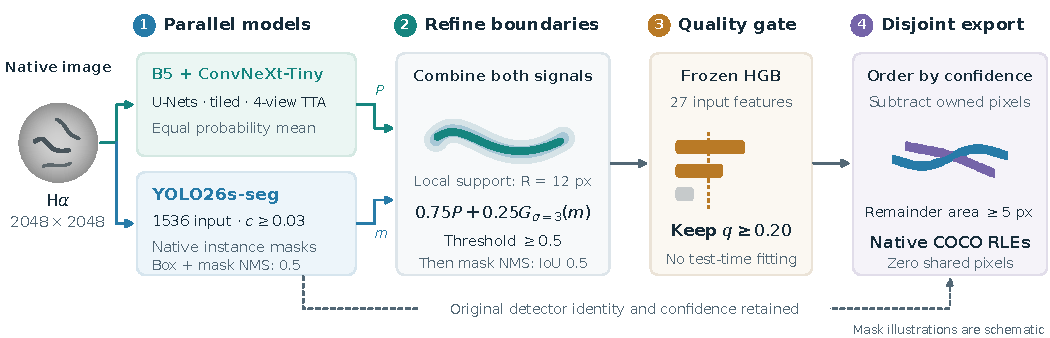
\includegraphics[width=\textwidth]{own_hybrid_submission_pipeline.pdf}
\captionof{figure}{Fixed hybrid inference. Two model branches feed boundary refinement, a frozen quality gate, and confidence-ordered pixel ownership. Illustrative masks are schematic. Base networks exclude the evaluated fold in local comparisons; deployment uses all official TRAIN images.}
\Description{Parallel detector and semantic U-Net branches converge on support-constrained boundary refinement. A frozen 27-feature quality model filters instances. Export preserves original detector confidence and identity, removes already-owned pixels, and encodes disjoint native masks. The miniature masks are illustrative schematics, not observations.}
\label{fig:pipeline}
\end{center}
}]
\section{Own Models and Fixed Inference Recipes}
\subsection{Semantic ensemble}
U-Nets~\cite{ronneberger2015unet} use EfficientNet-B5~\cite{tan2019efficientnet}/ConvNeXt-Tiny~\cite{liu2022convnext} encoders (ResNet34~\cite{he2016resnet}: reference). Grayscale is triplicated and normalized in-network. One random annotator supplies foreground union and auxiliary union of separately closed instances; auxiliary-threshold grouping is disabled.

B5/ConvNeXt: $768^2$ crops, batch 4, 40 epochs of 400 scheduled batches. AdamW: learning rate $6\times10^{-4}$, encoder factor 0.2, weight decay $10^{-4}$, cosine decay, EMA 0.999. Positive-centered crops: probability 0.7; scale/orientation/intensity augmentation. Foreground/auxiliary losses are BCE plus $0.5$ soft Dice, weighted $1:0.3$; empty targets use BCE. Independent folds start from generic weights. F1 B5/ConvNeXt skip 7/10 FP16 updates (scheduled batches $\neq$ optimizer updates).

Native inference: $768^2$ tiles, stride 512, batch 4, four inverse-aligned views (identity, horizontal, vertical, both flips). Separable raised-cosine window factors are individually clipped at 0.05. Float16 member caches: equal float32 mean, rounded to float16 before features. B5/ConvNeXt and R34/B5/ConvNeXt are the two-/three-member semantic ensembles, distinct from the hybrid.

Semantic-only instances use foreground threshold 0.35, elliptical closing radius 5 for connectivity/identity, minimum area 60 pixels, and $q\geq0.20$. Closing-added pixels are removed; output masks are disjoint.

\subsection{S60 detector and boundary adjustment}
YOLO26s-seg~\cite{ultralytics2026yolo}: generic COCO weights; 60 epochs on per-annotator image copies excluding fold 0. Executed settings, not defaults: size 1536, batch/nominal batch 8, AdamW rate 0.001, cosine decay, BF16, seed 2026, mask ratio 2, separate instance targets. Final-60 F1/F2: FP16, batch 2, nominal batch 8.

One-to-many inference (end-to-end disabled): size 1536, raw confidence floor 0.03, box NMS IoU 0.5, maximum 100 detections, native $2048^2$ masks. Confidence-ordered mask NMS IoU 0.5 removes duplicates; discard masks below five native pixels. Only the confidence comparison additionally requires confidence 0.20.

For binary instance $m$, the hybrid uses native B5/ConvNeXt foreground mean $P$:
\begin{equation}
\widetilde m=\ind[0.75P+0.25G_{\sigma=3}(m)\geq0.5]
\;\cap\;\operatorname{dilate}_{R=12}(m).
\label{eq:refine}
\end{equation}
Gaussian blur/elliptical dilation: $25\times25$ kernels, constant-zero borders, mask bounding box expanded by 12 pixels. Original detection identity/confidence persist; disconnected pieces remain one instance. Second confidence-ordered mask NMS IoU 0.5 precedes $q\geq0.20$; no extra detector-confidence cutoff.

\textbf{Disjoint export.} Stable descending original detector confidence (ties preserve selection order): subtract owned pixels; keep remainders of at least five pixels, dropped ones claim none. Disconnected pieces retain one source identity. No added pixels, morphology, NMS, quality reranking, or threshold search. Verify summed mask area equals union area per image.

\subsection{Quality estimation with fixed date meta-folds}
Semantic candidates use 26 size/shape, location, probability, auxiliary, grayscale, and contrast features; hybrids add original YOLO confidence. No inference feature uses annotations. Training utility:
\begin{equation}
y_j=\frac1{A_i}\sum_{a=1}^{A_i}\sum_{g\in G_{ia}}
u(p_j,g)\ind[u(p_j,g)>0.5],
\end{equation}
Candidate weight $A_i$ is the annotator-record count. This utility is not a calibrated probability of scientific validity.

Histogram gradient boosting uses 180 iterations, eight leaves, minimum leaf size 30, learning rate 0.05, $L_2=10$, seed 2026, no early stopping. Five-way cross-fitting holds out whole date groups using the original same-base-fold R34 map, independent of candidate-pool counts. Comparisons fix $q=0.20$. Deployment uses a separate final regressor fitted to all development candidates; its in-sample predictions are never reported as held-out.

\clearpage
\section{Results, Uncertainty, and Negative Findings}
\begin{table}[t]
\caption{Native semantic PQ at fixed q20. F0 is reused development; F1/F2 use independently trained base models and frozen same-fold quality maps.}
\label{tab:semantic}
\small
\begin{tabularx}{\columnwidth}{@{}Xrrr@{}}
\toprule
Semantic recipe & F0 & F1 & F2\\
\midrule
R34 reference & .424498 & .440940 & .421995\\
ConvNeXt-Tiny & .439477 & .450784 & .431664\\
EfficientNet-B5 & .434239 & .459311 & .428195\\
Equal B5/ConvNeXt & .441420 & .455338 & .437008\\
Equal R34/B5/ConvNeXt & .440859 & .460263 & .435404\\
\bottomrule
\end{tabularx}
\end{table}

\subsection{Semantic and complete-hybrid confirmation}
All four fixed semantic alternatives improve on R34 in F1 and F2 (Table~\ref{tab:semantic}). The F2 pair-minus-R34 difference is $+0.015013$, with conditional 95\% interval $[0.001728,0.028107]$. The three-member mean leads the pair on F1 but trails it on F2. Earlier descriptive F0/F1 pooling gave three-member PQ 0.450559 versus pair 0.448370; its difference interval included zero. We retain the pair without asserting universal superiority.

Paired bootstrap draws resample whole observation-date groups, then recompute Equation~\ref{eq:pq} from summed counts: 10,000 draws, seed 2026. These intervals condition on fixed predictions and exclude training and experiment-selection variability.

\begin{table}[t]
\caption{Fixed S60/equal-B5--ConvNeXt/q20 hybrids with confidence-disjoint export. F1/F2 gains are relative to their same-fold semantic pair. Pooled PQ uses summed counts, not averaged fold PQ.}
\label{tab:s60}
\small
\begin{tabularx}{\columnwidth}{@{}Xrrr@{}}
\toprule
Data & Hybrid PQ & Pair PQ & Difference\\
\midrule
F0 development & .456481 & .441420 & +.015061\\
F1 confirmation & .469083 & .455338 & +.013746\\
F2 confirmation & .444824 & .437008 & +.007816\\
F1+F2 descriptive & .455972 & .445493 & +.010480\\
\bottomrule
\end{tabularx}
\end{table}

The F1 hybrid has TP/FP/FN 1,025/421/528; F2 has 1,162/573/630. Each improves on its semantic pair in point estimate, but individual intervals include zero: F1 $[-0.001416,0.027241]$, F2 $[-0.002177,0.018030]$. The original same-fold meta-maps, geometry, q20, and pixel-ownership rule are fixed; no new threshold search is used.

Pooling the existing F1/F2 counts covers 283 distinct images and 121 disjoint date groups. Hybrid TP/FP/FN are 2,187/994/1,158, versus pair 2,166/1,130/1,179. The PQ difference is $+0.010480$, interval $[0.001784,0.018965]$: mainly fewer FP, with 21 additional matches. This is \emph{descriptive conditional evidence}; it does not adjust for repeated recipe selection or establish an untouched evaluation of a selected winner.

\subsection{Compliant fold-0 development evidence}
The fixed ownership correction changes 923 overlapping selections into 906 disjoint masks: PQ 0.456914 becomes 0.456481. Corrected IoU sum is 691.340436, TP/FP/FN 1,012/438/567. The difference interval $[-0.003564,0.002888]$ checks a required format correction on reused data. The old output is ineligible; neither score belongs to the all-data S20 checkpoint.

\begin{figure}[t]
\centering
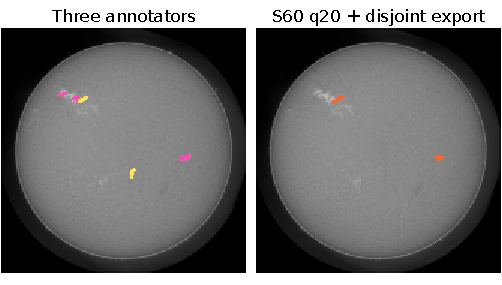
\includegraphics[width=\columnwidth]{own_hybrid_disjoint_validation.pdf}
\caption{Official TRAIN image 20110301082654Uh, fold 0: the lexicographically first image with at least two annotation records, chosen without scores. Left: three experts' contours (cyan, magenta, yellow; 1/4/2 instances). Right: existing S60 hybrid out-of-fold selections after fixed disjoint ownership. Different boundaries illustrate disagreement; this single deterministic example does not establish accuracy.}
\Description{Two views of the same solar disk show three annotators' filament boundaries and the existing compliant S60 hybrid predictions, without any test labels.}
\label{fig:example}
\end{figure}

\subsection{Changes that were not promoted}
On compliant F0 output, fixed 3,000-step SAM refinement reduced PQ from 0.456481 to 0.449749: difference $-0.006732$, interval $[-0.011560,-0.002218]$. Matched-mask IoU rose slightly, but TP fell and FP rose; the branch stopped.

Replacing the hybrid semantic input with ConvNeXt-V2 Base alone or an equal B5/ConvNeXt/Base mean gave 0.457575/0.458522. Gains $+0.001094/+0.002041$ have intervals crossing zero; neither was promoted. A single F0+F1 pooled quality fit gave F2 transfer PQ 0.447109 versus frozen-F0 transfer 0.446693: $+0.000416$, interval $[-0.003134,0.003699]$. This study is \emph{non-nested}: calibration-feature base models had trained on F2 images. No direct F2 targets entered that fit, but this is not independent outer-fold validation; deployment quality is unchanged.

Earlier size-2048, CLAHE, and instance-pool fusion follow-ups were negative or uncertain. Size 2048 reduced historical raw PQ 0.419095 to 0.400190; three-source instance fusion reached 0.436436 versus probability-mean 0.440859 with more FP. These findings concern tested recipes, not general claims against these methods.

\clearpage
\section{Accepted Candidate and Verified Reproduction}
\subsection{All-data training and public result}
B5/ConvNeXt continue from fold-0 EMA weights on all 707 training images for $20\times200$ scheduled batches, with fresh optimizer/EMA, rate $2\times10^{-4}$, and two/four skipped FP16 updates. S20 continues from S60 for 20 all-data epochs with fresh optimizer/EMA and rate 0.0002: final epoch 19, 2,900 EMA updates. None has a held-out score.

Deployment retains the equal B5/ConvNeXt mean, original F0 27-feature final quality model (\code{05ef8e57}), q20, and disjoint export. Membership and exported tensors are verified; test predictions never refit the quality model.

The accepted CSV has \textbf{1,219 disjoint masks across 180 test images}, SHA-256 prefix \code{9dd513669eee8b12}. Submission 58287816 was verified COMPLETE at 00:06:52 UTC, 13 November 2026: \textbf{public 0.40}. The earlier public best was 0.38 from an attributed public YOLO26x model~\cite{hdjojo2026}.

Separately, generic-COCO-initialized S60 trained on all 707 images using two T4 ranks, global/nominal batch 4/8, and FP16. Final-60 state/history checks passed. Unchanged semantics, quality, and export yield 1,206 masks (\code{61b019b8}). Submission 58293729 was verified COMPLETE at 03:40:15 UTC with \textbf{public 0.39}. S20 remains the selected candidate; no new public release or full reproduction of S60 is claimed.

\subsection{Numerical inference and reproduction}
After an earlier numerical mismatch, semantic inference uses fresh workers, native CUDA BF16, and float32 channels-last weights. Workers set cuBLAS to \code{:4096:8} before importing PyTorch, then disable cuDNN benchmarking and enable cuDNN deterministic behavior and strict deterministic algorithms. Matrix TF32 is off; cuDNN TF32 is on. Tile/TTA/rounding arithmetic is unchanged; precision fallback is forbidden.

The separate detector starts with CUBLAS unset and deterministic flags false. Its native constructor sets CUBLAS to \code{:4096:8}; FP32 inference is unchanged. An earlier run matched all 180 detector files but failed the old CUBLAS assertion. V3.1 corrects that assertion/reporting; failed evidence is preserved.

A fresh local v3.1 clone reproduced \code{9dd51366} byte-exactly: 180 images, 1,219 masks, 2,486.81 seconds excluding archive restoration. Independent CPU checks verified 180 detector files, 540 arrays, exact means, features/scores, source identities/confidences, R12, RLEs, and zero overlap. Processes exited cleanly; no test annotations were used.

Three notebook code cells ran as plain Python in an existing \code{.venv-repro} on GB10: no fresh installation, Jupyter kernel, new-machine, or cross-GPU proof. V3.2 preserves numeric sources/archives. Strict equality is default; explicit report-only mode records differences while retaining input/weight/source, backend, shape/finiteness, identity/R12, and disjointness guards. Nineteen CPU contracts and existing-output compatibility checks passed; no additional v3.2 GPU run is claimed.

Code and weights: \href{https://github.com/Tps-F/filament-segmentation-2026}{\nolinkurl{github.com/Tps-F/filament-segmentation-2026}}. Verified tag: \code{v3.1-verified}; code commit: \code{4981db24}.

The unchanged template uses a documented MIT-licensed derivative~\cite{pawar2026template}; official Overleaf byte identity is unverified.

% BEGIN PRESERVED ORGANIZER ACKNOWLEDGMENT (pinned derivative; see template_provenance.json)
\section{Acknowledgment}\label{sec:acknowledgment}
The organization of the Filament Segmentation Challenge 2026 is partially supported by the U.S. National Science Foundation (NSF) under Grant No. 2209912 and 2433781, directorate for Computer and Information Science and Engineering (CSE), and Office of Advanced Cyberinfrastructure (OAC), and Grant No. 2511630, AST Division Of Astronomical Sciences and MPS Directorate for Mathematical and Physical Sciences.

The Filament Segmentation Challenge 2026 is sponsored by the U.S. National Science Foundation (NSF) National Solar Observatory (NSO).

This work utilizes GONG data obtained by the NSO Integrated Synoptic Program, managed by the National Solar Observatory, which is operated by the Association of Universities for Research in Astronomy (AURA), Inc. under a cooperative agreement with the National Science Foundation and with contribution from the National Oceanic and Atmospheric Administration. The GONG network of instruments is hosted by the Big Bear Solar Observatory, High Altitude Observatory, Learmonth Solar Observatory, Udaipur Solar Observatory, Instituto de Astrofísica de Canarias, and Cerro Tololo Interamerican Observatory.
% END PRESERVED ORGANIZER ACKNOWLEDGMENT

\bibliographystyle{ACM-Reference-Format}
\bibliography{references,own_hybrid_references}
\end{document}
